\begin{figure}[h!]
	\centering
	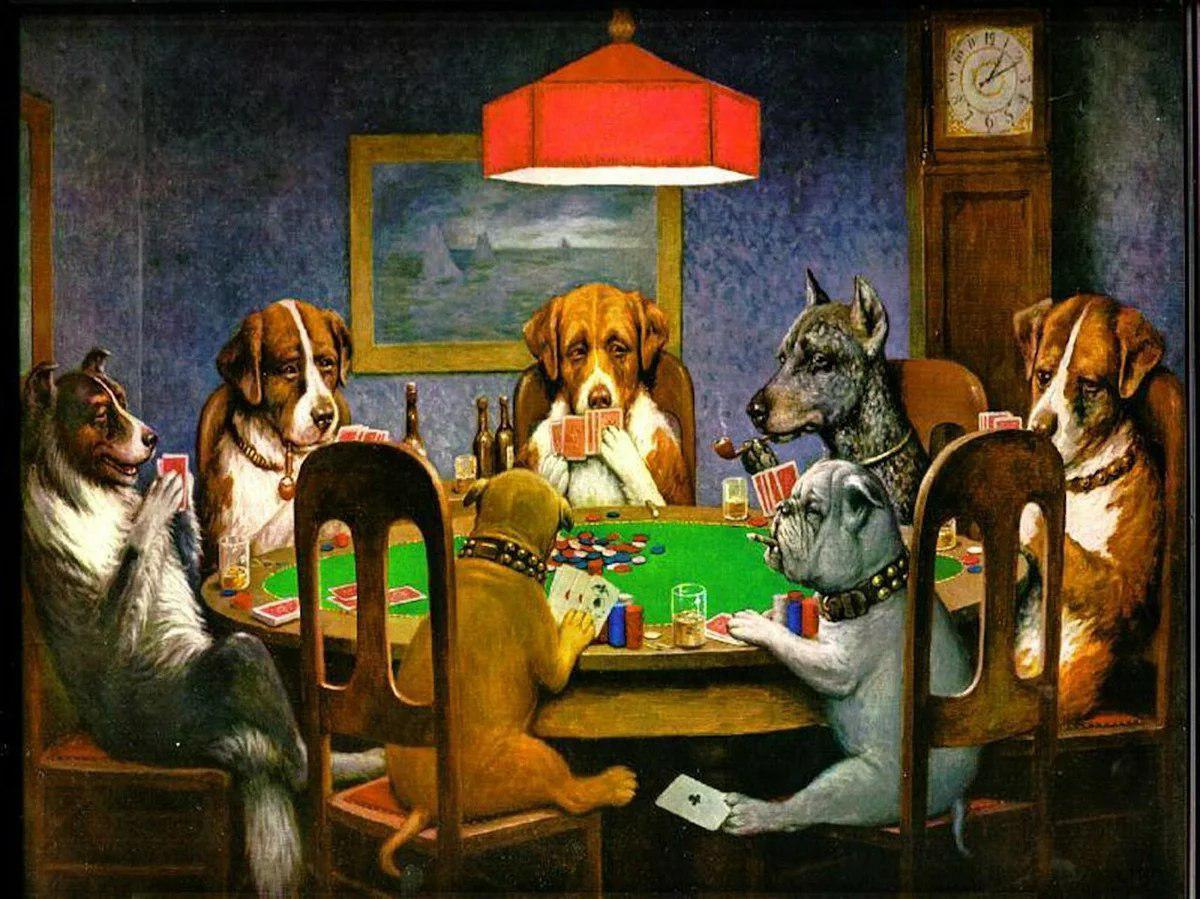
\includegraphics[width=0.8\linewidth, keepaspectratio]{poker.jpg}
\end{figure}

Как-то раз собрались собаки благородных пород за игрой в покер. 
Непроницаемые лица, дерзкие и подозревающие взгляды, запах мясных палочек и хруст говяжьих подушечек – все это было за круглым столом. 
Френки, молодой и уверенный в себе мопс, попал на сие мероприятие впервые. 
Он все силы потратил на получение приглашения на игру в столь элитном обществе, что не успел научится должным образом играть, поэтому он и нанял Вас. 
Помогите Френки выиграть в элитный собачий покер. Для выигрыша в покере необходимо владеть самой дорогой комбинацией. 
Необходимо сообщать Френки по маленькому наушнику, какая комбинация у него сейчас на руках. 
Игроки всегда владеют 5 картами, если они все одинаковые необходимо сообщить Френки, что кто-то мухлюет, так как это невозможно (\texttt{''Impossible``}). 
Если 4 карты одинаковы, то такая комбинация называется \texttt{``Four of a Kind''}. 
Если есть одинаковая тройка карт и пара, то \texttt{``Full House''}. 
Если одинаковы 3 карты, то \texttt{``Three of a Kind''}, 2 пары одинаковых~---~\texttt{``Two Pairs''}, 2 одинаковые карты~---~\texttt{``One Pair''}. 
Если все 5 карт имеют последовательные значения, то \texttt{``Straight''}. 
Если же на руках у Френки нет никакой удачной комбинации, то необходимо сообщить ему короткое кодовое слово \texttt{``Nothing''}.

\InputFile
\noindent

На вход подается 5 карт, с возможными значениями $[1 \ldots 13]$. Значения карт передаются через пробел.

\OutputFile
\noindent

Вывести результат анализа карт на лапах Фрэнки.

\SAMPLES